
\chapter{Knjižnica in gradniki za Orange}

V okviru diplomske naloge smo razvili tri ločene komponente za programerje in
končne uporabnike programa Orange. Prva komponenta je
dostopna kot samostojni paket 
\verb|simple_wbd|\fnurl{https://pypi.python.org/pypi/simple_wbd/0.5.0}. 
Druga in tretja komponenti pa sta zdru"zeni v paketu
\verb|orange3-datasets|\fnurl{https://pypi.python.org/pypi/Orange3-Datasets/0.1.3}

Prva komponenta je programska knjižnica \verb|simple_wbd|, ki
omogoča enostaven dostop do programskega vmesnika indikatorjev in podnebnih
podatkov Svetovne banke. Ta knjižnica je narejena s čim manj odvisnosti in je 
% TODO ali je python z veliko
namenjena splošni uporabi v Python programih. Poudarka pri zasnovi knjižnice 
\verb|simple_wbd| sta predvsem enostavnost razsiritve in zanesljivost. Ta cilja
dosežemo z mehanizmom za vključevanje lastne kode v komponente knjižnice
in mehanizmi za popravljanje ali odstranjevanje pokvarjenih podatkov.

Drugi sestavni del je razširitev knjižnice \verb|simple_wbd| s 
funkcionalnostmi, potrebnimi za lažje delo v programu Orange. To predvsem 
zavzema pretvorbo pridobljenih podatkov v podatkovno tabelo Orange in tabelo 
numpy. Ta sklop je namenjen skriptnemu delu s programom Orange 
\cite{orange_scripting} in je dostopen
kot \verb|api_wrapper| Python modul znotraj paketa \verb|orangecontrib.wbd|.

Tretji sestavni del je grafični vmesnik za uporabo \verb|api_wrapper| modula.
Namen grafičnega vmesnika je omogočiti ne-programerjem dostop do podatkov 
programskega vmesnika Svetovne banke znotraj programa Orange za namen obdelave,
analize in iskanja zakonitosti v podatkih.

\section{Knjižnica simple\_wbd}

Knjižnica \verb|simple_wbd| programerjem olajša dostop do podatkov 
programskega vmesnika Svetovne banke. Glavna lastnost te knjižnice je 
združevanje večjega števila zahtev po podatkih in enostavna predstavitev 
prejetih podatkov. Druga lastnost je pretvorba podatkov iz več dimenzij v 
dvo-dimenzionalno polje, primerno za uporabo v programu Orange. Glavna 
razreda te knjižnice sta \verb|IndicatorAPI| in \verb|ClimateAPI|. Prvi 
omogoča pridobivanje podatkov iz programskega vmesnika indikatorjev, drugi pa 
s programskega vmesnika podnebnih meritev.


Čeprav za dostop do programskega vmesnika Svetovne banke že obstajajo 
rešitve kot sta knjižnici 
\verb|wbdata|\fnurl{https://pypi.python.org/pypi/wbdata} in
\verb|wbpy|\fnurl{https://pypi.python.org/pypi/wbpy/2.0.1}, smo se odločili
za lastno implementacijo podobne knjižnice. Glavni razlog za to je, da
obstoječe rešitve poskušajo čim bolj natančno predstaviti programski
vmesnik Svetovne banke, ne pa olajšati dostop do čim večje količine
podatkov.

Za potrebe te knjižnice smo razvili lastno rešitev za predpomnenje poizvedb,
saj so se bolj splošne rešitve, kot na primer
\verb|vcrpy|\fnurl{https://pypi.python.org/pypi/vcrpy/1.10.0} in
\verb|requests-cache|\fnurl{https://pypi.python.org/pypi/requests-cache}, 
izkazale za prepočasne ko delamo z večjimi količinami podatkov. Naša
rešitev za predpomnenje izkorišča dejstvo da je vsaka poizvedba določena le
z naslovom URL, in da so vsi odgovori oblike JSON. Za vsak URL naredimo novo
datoteko v sistemskem začasnem imeniku, v kateri hranimo serializirane JSON
podatke. Ker se podatki na programskem vmesniku Svetovne banke redko
posodabljajo, smo za čas veljavnosti začasnih datotek izbrali en teden.

% NOTE: serailizacija je baje uredu beseda:
% http://eprints.fri.uni-lj.si/2711/1/63100205-VALENTIN_KRAGELJ-Pregled_in_analiza_tehnologij_za_serializacijo_objektov.pdf

% server query je ful omojen (retarded) mi mamo bolsiga v guiju 

%% % moznost razsiritve z dedovanjem dataset razreda.
%% % 
%% 
%% - omogoča pridobivanje vrednosti za filtre:
%%     - indicator api: drzave in agregati, indikatorji
%%     - climate api: drzave, tipi podatkov, meritveno obdobje 
%% 
%% - Zahteva za podatke vraca dataset objekt ki ponuja surove podatke, ali pa eno
%%   drugo obliko. 2D array ali pa dict.
%% 
%% - Dataset razred lahko tudi poljubno razsirimo.



\subsection{Razred IndicatorAPI}

\verb|IndicatorAPI| je razred namenjen pridobivanju podatkov indikatorjev
razvoja držav. Ker ima programski vmesnik Svetovne banke omejitev koliko 
podatkov lahko prenesemo z eno poizvedbo in nam dovoli tvoriti poizvedbe le za
en indikator na enkrat, smo napisali razred, ki v ozadju tvori in izvede
poizvedbe za vse strani vseh zahtevanih indikatorjev. To poskrbi tako da se po
prvi poizvedbi za en indikator sprehodi čez število preostalih strani 
(Primer \ref{basic_response}), ki so na voljo, in pridobljene podatke večih
strani združi in predstavi kot rezultat ene same poizvedbe. Ta postopek ponovi
za vse zahtevane indikatorje, in njihove rezultate vrne v obliki slovarja, ki 
ima za ključ kodo indikatorja posamezne zahteve.

Poleg tega da skrbi za prenos vseh strani podatkov, tudi beleži število 
izvedenih in število potrebnih poizvedb za celoten prenos. Ta števila se
lahko uporablja za prikaz napredka prenosa podatkov.


Za namene razreda \verb|IndicatorAPI| smo v knjižnici \verb|simple_wbd|
razvili mehanizme za odpravo nekaterih napak omenjenih v poglavju 
\ref{api_gotchas}.

Pri manjkajočih vrednostih držav v poizvedbah za podatke indikatorjev,
poskušamo določiti pravilne vrednosti. To naredimo s pomočjo dveh
slovarjev: prvi slika kode držav v imena, drugi pa imena držav v kode. V
primeru manjkajoče vrednosti kode ali imena, poskušamo to prebrati iz enega
od naštetih slovarjev. Če nam ne uspe ugotoviti manjkajočih vrednosti,
trenutni vnos odstranimo iz rezultata poizvedbe.

Drugi tip napak, ki ga lahko delno popravimo, so napačne vrednosti v polju
\verb|date| v poizvedbah za podatke indikatorjev. Ker lahko v temu polju
pričakujemo poljubno besedilo, dela naš pretvornik za polje \verb|date| v 
datum, tako da poskuša v datum pretvoriti čim daljšo predpono besedila.
Če nam ne uspe besedila pretvoriti v veljaven datum, trenutni vnos odstranimo
iz rezultata poizvedbe.


\ \\
Glavne metode ki jih ponuja razred IndicatorAPI so:

\begin{description}  
\item [get\_indicators] za pridobivanje seznama indikatorjev s kodami, imeni
      in opisi,
\item [get\_countries] za pridobivanje seznama držav z metapodatki,
\item [get\_dataset] za pridobivanje instance razreda \verb|IndicatorDataset|,
      ki vsebuje podatkov indikatorjev.
\end{description}

Ena izmed lastnosti razreda \verb|IndicatorAPI| je ta da mu lahko ob
inicializaciji podamo razred v katerem "zelimo prejeti rezultat poizvedbe. Ta
razred mora dedovati od osnovnega razreda \verb|IndicatorDataset|. Na ta
na"cin lahko enostavno raz"sirimo funkcionalnost \verb|simple_wbd| knji"znice.
V primeru \ref{indicator_api_extend} vidimo en na"cin za raz"siritev razreda 
\verb|IndicatorDataset| tako da uporabniku razreda \verb|MyIndicatorAPI| ni
potrebno izrecno podati razreda \verb|IndicatorDataset| v konstruktor.

\begin{snippet}
\begin{center}
\begin{lstlisting}
class MyIndicatorDataset(simple_wbd.IndicatorDataset):
    
    def as_numpy(self):
        raise NotImplemented()
    
    def as_orange_table(self):
        raise NotImplemented()

class MyIndicatorAPI(simple_wbd.IndicatorAPI):

    def __init__(self):
        super().__init__(MyIndicatorDataset)
\end{lstlisting}
\end{center}
\caption[some]{Primer raz"siritve osnovnega razreda rezultatov poizvedb.}
\label{indicator_api_extend}
\end{snippet} 


\subsubsection{Razred IndicatorDataset}

Razred \verb|IndicatorDataset| je osnovni razred v katerem dobimo zahtevane 
podatke indikatorjev. Ta razred vsebuje vse potrebne metode in podatke za 
predstavitev rezultatov programskega vmesnika, na dva načina: kot slovar
rezultatov poizvedb za posamezen indikator in dvo dimenzionalen seznam. 
Posamezna vrednost v teh podatkih je določena z državo, časovno komponento in 
kodo indikatorja. 

Podatke lahko predstavimo kot dvodimenzionalno polje v dveh oblikah: kot
"casovne vrste ali kot podatki dr"zav. Obliko predstavitve izberemo s
parametrom \verb|time_series| metode \verb|as_list|. Za predstavitev obeh oblik
je prva vrstica polja uporabljena kot naslovna vrstica, ki opisuje podatke v 
stolpcih.

Ko uporabljavo obliko "casovnih vrst, so elementi prve vrstice kartezi"cni
produkt kod indikatorjev in dr"zav. V prvem stolpcu polja pa imamo casovno
komponento podatkov. Na ta na"cin so vsi ostali elementi polja dolo"ceni s 
casovno komponento, dr"zavo in kodo indikatorja.

Ko dostopamo do dvodimezionalnega polja ki predstavlja podatke dr"zav, pa je v
prvi vrstici kartezi"cni produkt kod indikatorjev in casovne komponente. Prvi
stolpec v tej predstavitvi vsebuje imena drzav. Za razliko od predstavitve v 
obliki "casovnih vrst, v to polje vstavimo se dodatne stolpce ki vsebujejo
metapodatke drzav iz primera \ref{country_response}: regija \verb|region|, administrativna regija
\verb|adminregion|, vi"sina dohodka \verb|incomeLevel|, vrsta posojil
\verb|lendingType|, geografska "sirina \verb|latitude|, geografska dol"zina
\verb|longitude|. Tudi tukaj vsi ostali elementi dolo"ceni s casovno 
komponento, dr"zavo in kodo indikatorja. 

% \subsubsection{Primeri uporabe}
% 
% Razreda \verb|IndicatorAPI| in \verb|IndicatorDataset| 
% 
% 
% import simple_wbd
% api = simple_wbd.IndicatorAPI()
% seznam_indikatorjev = api.get_indicators()
% kode_indikatorjev = [indikator.get("id") for indikator in seznam_indikatorjev]
% indicator_dataset = api.get_dataset(kode_indikatorjev[:3])


\subsection{Razred ClimateAPI}

Razred \verb|ClimateAPI| olaj"sa dostop do podnebnih podatkov programskega
vmesnika Svetovne banke. Ta programski vmesnik dovoli poizvedbe po podatkih le 
ene vrste meritev za eno vrsto meritvenega obdobja in eno drzavo. Na"s razred 
naredi kartezi"cni produkt med vsemi zahtevanimi vrstami meritev, vrstami
meritvenih obdobij in dr"zavami. Nato iz tega zgradi in izvede vse poizvedbe 
in predstavi podatke kot enotni odgovor. V razredu \verb|ClimateAPI| hranimo 
tudi "stevilo vseh potrebnih poizvedb in "stevilo "ze izvedenih poizvedb, kar 
lahko uporabimo za prikaz napredka prenosa podatkov.



\subsubsection{Razred ClimateDataset}

Razred \verb|ClimateDataset| je osnovni razred v katerem dobimo zahtevane 
podatke podnebnih meritev. Ta razred vsebuje vse potrebne metode in podatke za 
predstavitev rezultatov programskega vmesnika, na dva glavna načina: kot
gnezden slovar in dvo dimenzionalen seznam. Posamezna vrednost v teh podatkih
je določena z državo, vrsta podatkov, in "casovno komponento. Poleg omenjenih
načinov predstavitve podatkov lahko dostopamo tudi do neobdelanih podatkov 
prejetih iz programskega vmesnika za vsako poizvedbo posebej.

"Casovna komponenta rezultata je sestavljena iz vrste meritvenega obdobja in 
za"cetkom obdobja meritve. Sestavljo "casovno komponento uporabljamo, da se 
izognemo dvoumnim primerom vrednosti za"cetka obdobja za letni in deseteletni 
interval meritev. Primera takih dveh "casovnih obdobij sta 
\verb|'decade - 1990'| in \verb|'year - 1990'|.


Do podatkov predstavljenih z gneznedim slovarjev lahko dostopamo preko funkcije
\verb|as_dict|. V tej funkciji zdru"zimo podatke poizvedb programskega
vmesnika v gnezden slovar s "stirimi nivoji gnezdenja: drzava, vrsta meritev,
vrsta meritvenega obdobja in obdobje meritve. Zadnji nivo gnezdenja pa vsebuje
vrednosti podnebnih meritev.

Pri predstavitvi podatkov kot dvodimenzionalno polje, moramo dve od treh
komponent podatkov (država \verb|'country'|, vrsta podatkov \verb|'type'|, 
in "casovna komponenta \verb|'interval'|)
zdru"ziti in ju skupaj prikazati v vrsticah ali stolpcih. Za razliko od razreda
\verb|IndicatorDataset|, ki podpira le dve obliki prikaza, lahko v razredu
\verb|ClimateDataset| sami dolo"cimo katere komponente bodo v stolpcih in
katere v vrsticah. Primer razli"cnih izborov komponent je prikazan v
\ref{list_configurations}. Spremenljivki \verb|list1| ind \verb|list2| iz
prej"snjega primera prikazujeta privzeto konfiguracijo, kjer imamo v stolpcih
kartezi"cni produkt vrst meritev in vrst meritvenih obdobij, v vrsticah pa
podatke dr"zave. Spremenljivka \verb|list4| prikazuje konfiguracija za
predstavitev v obliki "casovnih vrst.

\begin{snippet}
\begin{center}
\begin{lstlisting}
import simple_wbd

api = simple_wbd.ClimateAPI()                   
climate_dataset = api.get_instrumental(["svn", "usa", "aus"])

list1 = ds.as_list()
list2 = ds.as_list(columns=["type", "interval"])  # default  value
list3 = ds.as_list(columns=["type"])
list4 = ds.as_list(columns=["type", "country"]) 
list5 = ds.as_list(columns=["country"])
\end{lstlisting}
\end{center}
\cprotect
\caption{Prikaz nekaj mo"znih oblik dvodimezionalnega polja vrednosti.} 
\label{list_configurations}
\end{snippet} 



\section{Modul api\_wrapper}


Znotraj paketa \verb|orangecontrib.wbd| smo razvili modul \verb|api_wrapper| v
katerem smo raz"sirili razreda \verb|IndicatorDataset| in \verb|ClimateDataset|
na na"cin ki je prikazan v primeru \ref{indicator_api_extend}. Na"sa
raz"siritev obema razredoma doda metodi za pretvorbo podatkov v podatkovno 
tabelo Orange in tabelo numpy.

TODO: opis posameznih raz"siritev in primer skripte uporabe.




% % doda as orange table in as numpy obema indikator apiju in climate apiju.
% 
% 
% razširitev simple wbd vmesnikov z dedovanjem pravega dataset razreda.
% 
% 
% - razsiri as\_list v as\_numpy\_array ki tudi odstrani vse stolpce ki nimajo 
%   veljavne vrednosti.
% 
% - doda as orange table ki numpy array spremeni v orange tabelo.
%   - za indikator api doda se metapodatke drzav ko ne prikazujemo v obliki casovne vrste.
% 
% 
% api vrapper je tudi zelo uporaben za skriptno uporaba programa Orange 
% (referenca http://www.jmlr.org/papers/volume14/demsar13a/demsar13a.pdf)
% 
% in tukaj si lahko vsak programer sam oblikuje podatke v katerokoli zeljeno obliko.
% 
% 
% TODO: primer skripte
% 
% % from orangecontrib.wbd import api_wrapper
% % api = api_wrapper.IndicatorAPI()
% % seznam_indikatorjev = api.get_indicators()
% % kode_indikatorjev = [indikator.get("id") for indikator in seznam_indikatorjev]
% % indicator_dataset = api.get_dataset(kode_indikatorjev[:3])





\section{Graficni vmesnik}

Za namen tega diplomskega dela smo z dodatkom \verb|Orange3-DataSets|
grafi"cnemu vmesniku programa Orange, dodali novo skupino gradnikov imenovano
``Data Sets'' (Slika \ref{data_sets_group}). V okviru te naloge smo za skupino
``Data Sets'' izdelali dva lo"cena gradnika. Prvi gradnik se imenuje ``WB
Climate'' in nam preko grafi"cnega vmesnika omogo"ca dostop do pobnebnih 
podatkov Svetovne banke. Drugi gradnik pa se imenuje ``WB Indicators'' in nam
preko grafi"cnega vmesnika omogo"ca dostop do podatkov indikatorjev razvoja.
 
nova skupina data sets 
 - v katero je mogoce dodati nove gradnike za druge programske vmesnike.

2 gradnika - wb indicators in wb climate

- lazja uporaba apija
- vecja preglednost


za oba gradniko smo razvili in uporabili base class - skupni podatki

- razvili smo tudi gradnik za gnezned prikaz urejenih slovarjev.
  ta se uporablja za prikaz drzav po kontinentih v climate gradniku,
  in za prikaz drzav in skupin drzav in drugih agregatov v gradniku
  indicators.


za te gradnike smo tudi napisali enotske teste.


\begin{figure}
  \begin{center}
    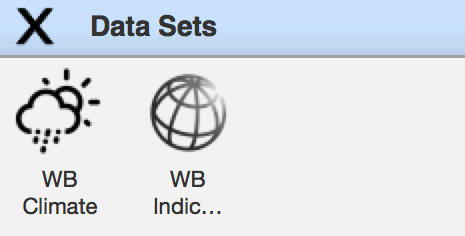
\includegraphics[width=4cm]{pic/data_sets_group.png}
  \end{center}
  \caption{Skupina gradnikov data sets}
  \label{data_sets_group}
\end{figure} 


\subsection{wb indicators gradnik}

za sestavo smo si pomagali z gradniki Orange.gui 

elementi gradnika

2 osnovna filtra: 

- izbor indikatorjev ki se pokazejo v seznamu all/common/featured 
  ki ustreza seznamu indikatorjev na strani: 
  all - vse (tudi nekateri ki jih na strani ni nastetih)
  common - http://data.worldbank.org/indicator?tab=all
  featured - http://data.worldbank.org/indicator?tab=featured
- text filter

gradnik ima sistem za prikaz (progress bar?) 

moznost izbire tipa izhoda (countries in time series - opis)

\begin{figure}
\begin{center}
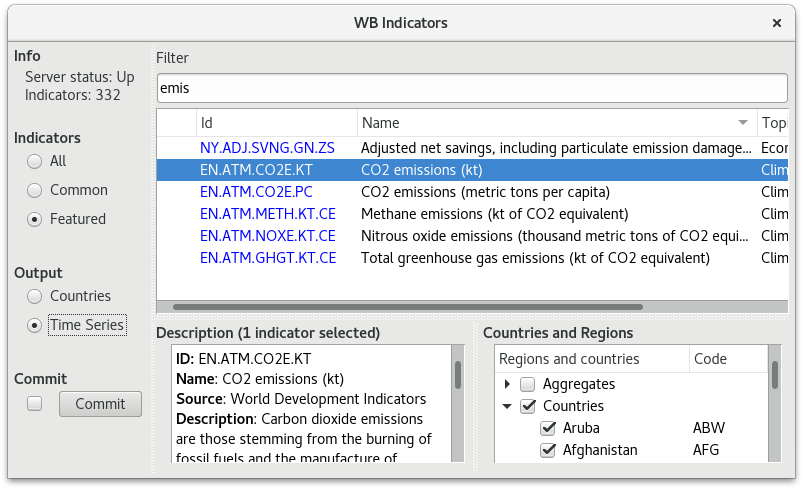
\includegraphics[width=12cm]{pic/co2_temp_indicator_selection.png}
\end{center}
\caption{Odločitveno drevo za izbor primerne metode.}
\label{co2_temp_indicator}
\end{figure} 



\subsection{wb climate gradnik}

dovoli izbiro posameznih drzav 

moznost izbire tipa izhoda (countries in time series - opis)
za razliko od indikator apija tukaj nismo dodali metapodatkov drzav 



\begin{figure}
\begin{center}
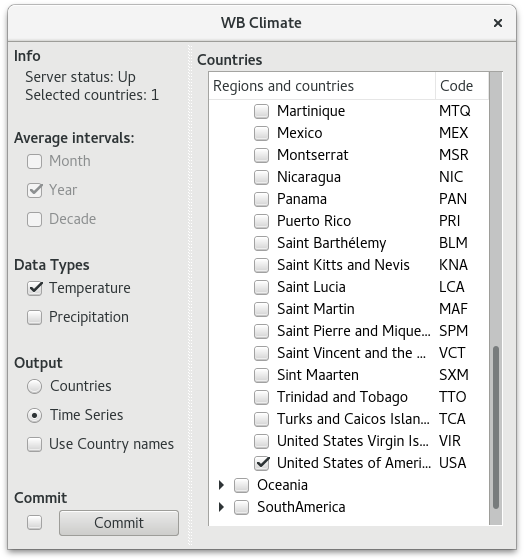
\includegraphics[width=12cm]{pic/co2_temp_climate_selection.png}
\end{center}
\caption{Odločitveno drevo za izbor primerne metode.}
\label{co2_temp_indicator}
\end{figure} 
